% !TeX root = ../main.tex
\section{Methodology}
\label{sec:methods}

The framework reconstructs stand-level rotational harvest histories through three components: STS construction, pixelwise windowed CuSum detection, and stand-level harvest-history reconstruction (Fig.~\ref{fig:workflow}). First, STS construction organizes monthly Sentinel-1 observations into track-consistent trajectories at fixed 30~m grid cells (Section~\ref{sec:s1_timeseries_representation}). Second, windowed CuSum identifies persistent negative backscatter shifts using overlapping context windows, central decision intervals, and window-specific permutation testing (Section~\ref{sec:windowed_cusum}). Third, TDA consolidates staggered pixelwise detections into stand-level harvest events, while STP resolves spatial harvesting progression within individual events (Section~\ref{sec:stand_history_reconstruction}). Experimental design and accuracy assessment are described in Section~\ref{sec:experimental_evaluation}.

% Reconstructing rotational harvesting from decadal SAR records requires identifying successive stand-replacing canopy removals and resolving their spatial and temporal patterns. Three characteristics of short-rotation plantations guide our methodological design. First, harvesting recurs on the same land, requiring fixed spatial units across which successive management cycles can be tracked. Second, repeated harvesting and rapid regrowth continuously alter canopy structure, rendering a single long-term baseline inadequate for detecting subsequent harvests. Third, harvesting often progresses asynchronously within a stand over several months; collapsing a stand into a single averaged trajectory obscures this progression, whereas treating each pixel independently fragments a single harvest into multiple events.

% To address these requirements, we developed a four-stage framework (Fig.~\ref{fig:workflow}(a--d)): (1) organizing Sentinel-1 observations into track-consistent spatial time series (STS) at 30~m pixel locations; (2) detecting persistent negative backscatter shifts at the pixel level using windowed CuSum (Fig.~\ref{fig:workflow}(a, b)); (3) consolidating pixelwise detections into stand-level harvest events via temporal detection aggregation (TDA; Fig.~\ref{fig:workflow}(c)) while resolving intra-event harvesting progression via spatial timing partitioning (STP; Fig.~\ref{fig:workflow}(d)); and (4) evaluating event recovery and dating accuracy against independent reference records before mapping national harvest dynamics.

\begin{figure*}[pos=!htbp]
    \centering
    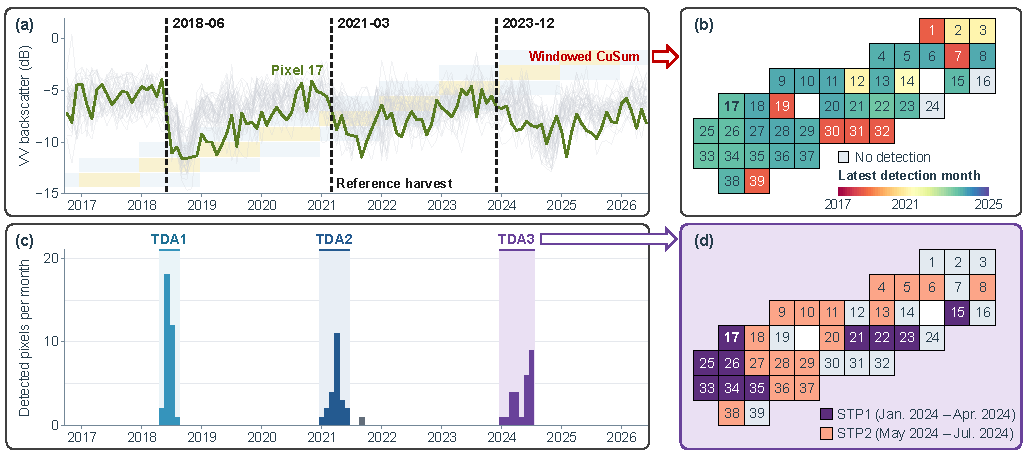
\includegraphics[width=\linewidth]{figures/fig02_workflow.pdf}
    \caption{Overview of the rotational harvest mapping framework, illustrated using inventory stand~22301. (a) Pixelwise windowed CuSum detection, showing 36-month context windows, 12-month decision intervals, and reference harvests. (b) Latest detection month per 30~m pixel during 2017--2025. (c) Three stand-level harvest events identified by temporal detection aggregation (TDA). (d) Intra-event timing groups identified by spatial timing partitioning (STP).}
    \label{fig:workflow}
\end{figure*}

% --------------------------------------------------
\subsection{Spatial time-series construction}
\label{sec:s1_timeseries_representation}

We represented each plantation stand as a spatially explicit set of long-term monthly pixelwise STS because harvesting recurs on the same land, requiring fixed spatial units across which successive management cycles can be tracked. Specifically, each STS links a track-consistent Sentinel-1 trajectory to a fixed 30~m grid cell~\citep{Guo2025SpatialAssociation} (Fig.~\ref{fig:sts_construction}(a--c)). Retaining individual pixel trajectories rather than averaging backscatter across stand polygons preserves both the temporal signatures of successive canopy changes and their spatial arrangement, providing the basis for subsequent pixelwise detection and stand-level harvest reconstruction.

\begin{figure*}[pos=!htbp]
    \centering
    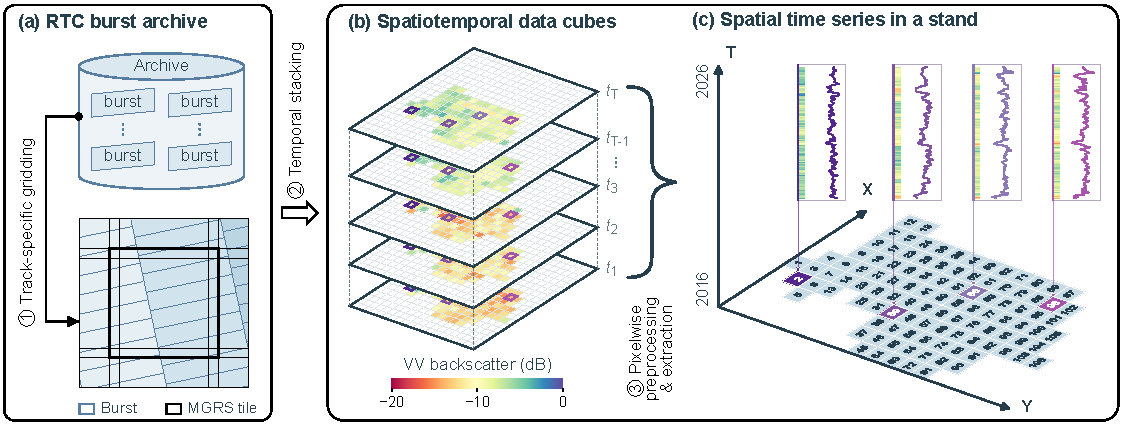
\includegraphics[width=\linewidth]{figures/fig03_sts_construction.pdf}
    \caption{Construction of 30~m spatial time series (STS) from Sentinel-1 RTC bursts. (a) RTC burst archive indexed to MGRS tiles by relative orbit (step~1). (b) Track-specific monthly spatiotemporal data cubes (step~2). (c) Pixelwise monthly VV trajectories extracted within stand polygons (step~3).}
    \label{fig:sts_construction}
\end{figure*}

Using the S1-GRiTS framework (Section~\ref{sec:satellitedata}), burst-level RTC-S1 images were organized by specific track on MGRS-aligned 30~m grids. For each grid cell and ascending track, valid linear-power $\gamma^{0}$ observations within each calendar month were summarized by their median and converted to decibels (dB). Maintaining each trajectory within a single relative orbit avoids mixing observations acquired under different viewing geometries~\citep{Navacchi2023RTCOrbit}. Where coverage from adjacent tracks or grid zones overlapped, the trajectory with the greatest number of jointly valid VV and VH months was retained at each location.

Grid cells whose centres fell within a plantation polygon were assigned to that stand. For stand $s$, this assignment defined a fixed set of $N_s$ pixels. All pixel trajectories were aligned to a uniform 126-month calendar from January 2016 to June 2026, with missing observations left unfilled. Monthly VV backscatter in dB, denoted $x_{u,t}$ for pixel $u$ and month $t$, served as the primary detection variable. VH was retained for polarization sensitivity analyses.

% --------------------------------------------------
\subsection{Pixelwise windowed CuSum detection}
\label{sec:windowed_cusum}

Repeated harvesting and rapid regrowth continuously alter canopy structure, rendering a single long-term baseline inadequate for detecting subsequent harvests. To address this challenge, we developed \textit{windowed CuSum}, a locally adaptive change-detection method for reconstructing recurrent harvest-related backscatter declines (Fig.~\ref{fig:windowed_cusum_concept}). It combines overlapping temporal contexts, non-overlapping decision intervals, and window-specific permutation testing. Overlapping windows renew local reference baselines as canopy conditions evolve across rotations, while central decision intervals assign candidate changes to distinct reporting periods. Window-specific permutation testing evaluates cumulative deviations against the temporal variability within each context window. Unlike recursive segmentation~\citep{Ygorra2023ReCuSum}, later detections do not depend on earlier detected change points.

\begin{figure*}[pos=!htbp]
    \centering
    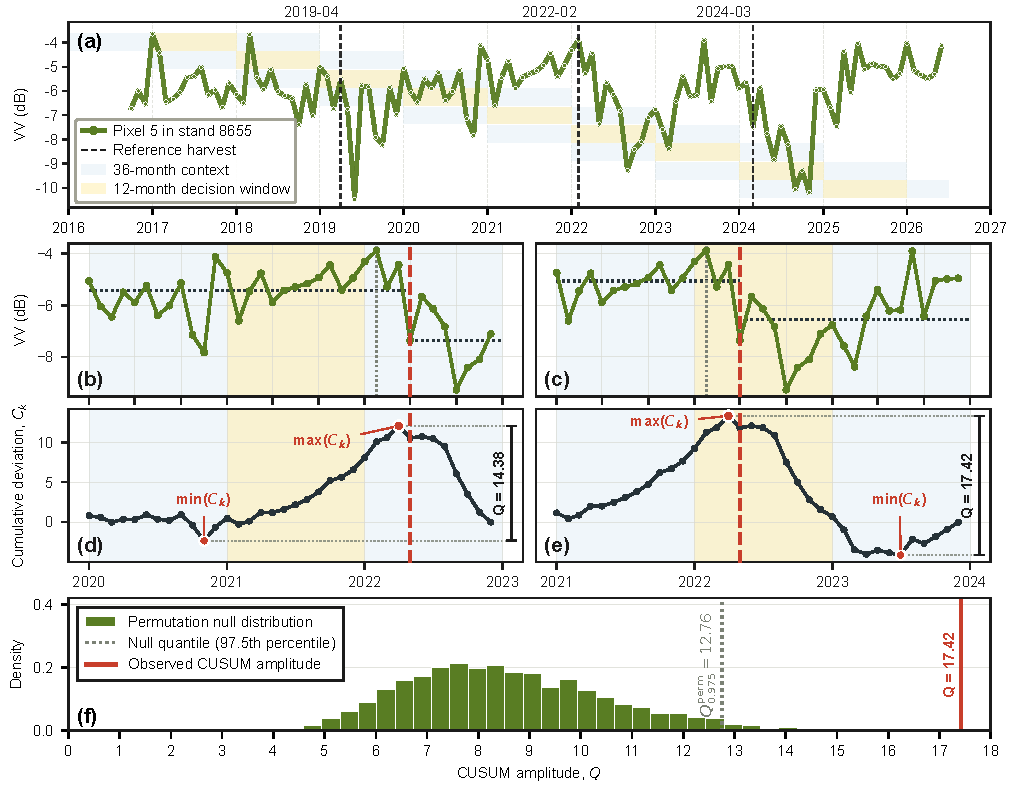
\includegraphics[width=\linewidth]{figures/fig04_windowed_cusum_concept.pdf}
    \caption{Principle of pixelwise windowed CuSum (Pixel~5, Stand~8655). (a) Monthly VV trajectory with overlapping 36-month context windows, central 12-month decision intervals, and reference harvests. (b,c) VV observations and pre-/post-shift means in two consecutive windows. (d,e) Cumulative deviations $C_k$ and full ranges $Q$, where the candidate falls outside the decision interval in (d) ($Q=14.38$) but enters testing in (e) ($Q=17.42$). (f) Permutation null distribution of $Q$, comparing observed $Q$ against the 97.5th percentile ($Q^{\mathrm{perm}}_{0.975}=12.76$).}
    \label{fig:windowed_cusum_concept}
\end{figure*}

We separated each context window $\mathcal{W}_j$ used for change estimation from its decision interval $\mathcal{D}_j$, within which candidates were eligible for reporting. As shown in Fig.~\ref{fig:windowed_cusum_concept}, the baseline used a 36-month context window ($W=36$), a central 12-month decision interval ($D=12$), and a 12-month advancement step ($S=12$). Each nominal window comprised the reporting year and its preceding and following years. Adjacent context windows therefore overlapped by 24 months, whereas decision intervals covered successive calendar years from 2017 to 2025 without overlap. The final context was truncated to January 2024--June 2026, retaining the full 2025 decision interval without shifting or padding the window. A window required at least 12 valid months under the joint VV--VH observation mask. All valid VV observations contributed to estimation in chronological order; missing months were not interpolated.

Within context window $\mathcal{W}_j$, let $t_1<\cdots<t_n$ denote the valid observation months for pixel $u$, with $z_i=x_{u,t_i}$ and $\bar z=n^{-1}\sum_{i=1}^{n}z_i$. We computed cumulative residuals and their full range as Equation~\eqref{eq:cusum_amplitude}.
\begin{equation}
    \begin{aligned}
        C_k &= \sum_{i=1}^{k}(z_i-\bar z),
        \qquad k=1,\ldots,n,\\
        Q &= \max_{1\leq k\leq n}C_k
             - \min_{1\leq k\leq n}C_k.
    \end{aligned}
    \label{eq:cusum_amplitude}
\end{equation}

A sustained decline produces predominantly positive deviations before the transition and negative deviations afterward, causing the cumulative sequence to rise and then fall. We selected its earliest global maximum and assigned the candidate date to the next valid observation month (Equation~\eqref{eq:candidate_date}). Thus, the candidate date denotes the first valid month after the cumulative peak, which need not be the next calendar month.
\begin{equation}
    \begin{aligned}
        k^* &=
        \min\left\{
            k\in\{1,\ldots,n\}:
            C_k=\max_{1\leq \ell\leq n}C_\ell
        \right\},\\
        \hat{\tau}_{u,j} &= t_{k^*+1},
        \qquad k^*<n.
    \end{aligned}
    \label{eq:candidate_date}
\end{equation}


A candidate proceeded to permutation testing only when $k^*<n$, $\hat{\tau}_{u,j}\in\mathcal{D}_j$, and $\bar z_{\mathrm{post}}<\bar z_{\mathrm{pre}}$. Here, $\bar z_{\mathrm{pre}}$ and $\bar z_{\mathrm{post}}$ are the means of $z_1,\ldots,z_{k^*}$ and $z_{k^*+1},\ldots,z_n$, respectively. Windows failing these conditions were skipped without searching for alternative peaks. For each qualifying window, we randomly reordered its $n$ valid values $B$ times and recomputed the CUSUM range:
\begin{equation}
    p_{\mathrm{perm}}
    =
    \frac{
        1+\sum_{b=1}^{B}
        \mathbf{1}\!\left\{
            Q_b^{\mathrm{perm}}\geq Q
        \right\}
    }{B+1},
    \label{eq:permutation_pvalue}
\end{equation}
where $Q_b^{\mathrm{perm}}$ is the CUSUM range computed from the $b$th permuted sequence and $\mathbf{1}\{\cdot\}$ is the indicator function~\citep{PhipsonSmyth2010Permutation}. This comparison evaluates the observed CUSUM range against a window-specific random-order distribution, rather than testing the candidate date itself. Permuted sequences were used only to recompute $Q$; candidate-date and directional screening were not repeated.

We initially used $B=3{,}999$ permutations, refining the total to $19{,}999$ when the initial $p_{\mathrm{perm}}\in[0.015,0.035]$ to improve precision near the acceptance threshold. Candidates were accepted when the final $p_{\mathrm{perm}}\leq\alpha_{\mathrm{ts}}$, with $\alpha_{\mathrm{ts}}=0.025$. This threshold applies to individual candidate windows and does not specify a record-wide false-alarm rate. Unrestricted permutation assumes exchangeability under the null and does not preserve temporal autocorrelation; sensitivity to this assumption was examined using calendar-block permutations (Section~\ref{sec:experimental_evaluation}). Selecting one candidate per window and using non-overlapping annual decision intervals allowed at most one accepted detection per pixel per reporting year. Detections in successive years were retained to reconstruct recurrent harvesting.

% ---------------------------------------------------------------------------
\subsection{Stand-level event aggregation and harvest-history mapping}
\label{sec:stand_history_reconstruction}

Harvesting often progresses asynchronously within a stand over several months. Collapsing a stand into a single averaged trajectory obscures this progression, whereas treating each pixel independently fragments a single harvest into multiple detections. In our framework, TDA consolidates staggered pixelwise detections into stand-level harvest events, while STP resolves the spatial organization of harvesting progression within each event (Fig.~\ref{fig:workflow}(c, d)).
% Harvest-history statistics were derived from TDA events; STP did not alter their number or representative dates.

For stand $s$ and month $t$, $A_{s,t}$ denotes the number of distinct pixels with accepted detections, and $V_{s,t}$ counts pixels with valid monthly inputs and context windows containing at least 12 valid months. Given the fixed stand pixel count $N_s$, monthly states were classified as shown in Equation~\eqref{eq:monthly_activity_state}.
\begin{equation}
    \mathrm{State}_{s,t} =
    \begin{cases}
        \text{active}, & A_{s,t}\geq 1,\\
        \text{observed non-detection}, & A_{s,t}=0,\; V_{s,t}\geq 0.5N_s,\\
        \text{unknown}, & \text{otherwise}.
    \end{cases}
    \label{eq:monthly_activity_state}
\end{equation}

Consecutive active months were grouped and merged across a single observed non-detection month. At least two consecutive observed non-detection months separated events; gaps containing unknown months without this separation remained unresolved. Components adjoining unresolved internal boundaries were not reported. The remaining components were retained as harvest events when distinct contributing pixels accounted for at least 20\% of $N_s$, including events censored at the observation-period edges. Each event was dated by the median of its contributing pixel--month detections, rounded to the nearest month. Repeated detections from the same pixel contributed to event dating but counted only once toward spatial support.

STP tested events with $N_s\geq25$ and at least 15 distinct contributing pixels. Spatial testing used the tile--track group with the most contributing pixels, requiring at least four pixels and three edge-sharing neighbour pairs. Within this group, neighbours were linked when their first-detection months differed by at most $\delta\in\{0,1,2\}$ months; connected components defined initial timing zones. For each tolerance, $J_\delta$ counted neighbour pairs crossing zone boundaries. We permuted first-detection months among fixed pixel locations 999 times, rebuilding zones at every tolerance for each permutation. The resulting counts $J_{\delta,b}$ supplied the null mean $\mu_\delta$ and standard deviation $\sigma_\delta$ in Equation~\eqref{eq:spatial_organization}.
\begin{equation}
    \begin{aligned}
        T_{\mathrm{obs}} &= \min_{\delta\in\{0,1,2\}} \frac{J_\delta-\mu_\delta}{\sigma_\delta},\\
        T_b &= \min_{\delta\in\{0,1,2\}} \frac{J_{\delta,b}-\mu_\delta}{\sigma_\delta},\\
        p_{\mathrm{sp}} &= \frac{1+\sum_{b=1}^{999}\mathbf{1}\!\left\{T_b\leq T_{\mathrm{obs}}\right\}}{1000}.
    \end{aligned}
    \label{eq:spatial_organization}
\end{equation}

Thus, observed and permuted statistics included the same tolerance search. Partitioning required positive null standard deviations at all tolerances, $T_{\mathrm{obs}}<0$, and $p_{\mathrm{sp}}\leq0.05$.

At the selected tolerance, zones with fewer than three pixels were merged into the temporally nearest larger zone based on median first-detection months. Zones were then ordered by their rounded median first-detection months and divided into timing groups at gaps exceeding two months. Partitions were retained only when at least two groups each contained at least 20\% of $N_s$; otherwise, the event remained unsplit. Group representative months followed the TDA dating rule, while the parent event's date remained unchanged.

Stand harvest frequency was the number of TDA events during 2017--2025. Annual and quarterly counts used representative event months, whereas inter-harvest intervals were measured between consecutive events' first-detection months. Counts were aggregated by canton, and intervals within each 10-km hexagon were summarized by their modal three-month bin, with ties flagged separately. Interval distributions were also compared across 1-km K\"oppen--Geiger climate zones~\citep{Beck2023KoppenGeiger}.


% =========================================================
\subsection{Experimental design and accuracy assessment}
\label{sec:experimental_evaluation}

We evaluated harvest-associated SAR backscatter responses, stand-level event detection and rotational-history recovery, component contributions and configuration sensitivity, and performance against alternative detectors. The reference catalogue comprised 1,049 dated harvest events across 459 stands during 2017--2025.

To characterize backscatter responses, observations were aligned to each reference harvest month (month $0$). Pixels were eligible if they had at least six valid observations in both VV and VH during months $-12$ to $-3$ and at least two during months $0$ to $+2$. For each eligible pixel, backscatter change was calculated as the post-harvest median minus the pre-harvest median. Reference events with eligible pixels covering at least 50\% of the stand's fixed membership were retained, yielding 978 events. Pixelwise changes were summarized by their median within each event, and event-aligned trajectories were summarized over months $-12$ to $+12$ relative to pre-harvest baselines. Pooled monthly backscatter observations from the plantation inventory provided distributional context. Uncertainty in event-level responses was estimated using 5,000 bootstrap resamples of 61 spatial blocks.

All detector configurations were evaluated using the same TDA and reference-matching rules. Within each stand, a detected event matched a reference harvest if its first-to-last detection span overlapped the reference month $\pm1$ month. One-to-one assignment maximized the number of matches. Precision, recall, and F1 were calculated from counts pooled across the 459 reference stands as shown in Equation~\eqref{eq:reference_agreement_metrics}.
\begin{equation}
    \begin{aligned}
        P_{\mathrm{ref}} &= \frac{M}{N_{\mathrm{det}}}, \qquad
        R_{\mathrm{ref}} = \frac{M}{N_{\mathrm{ref}}},\\
        F_{1,\mathrm{ref}} &= \frac{2M}{N_{\mathrm{det}}+N_{\mathrm{ref}}},
    \end{aligned}
    \label{eq:reference_agreement_metrics}
\end{equation}
where $M$ is the number of matched events, $N_{\mathrm{det}}$ the number of detected events, and $N_{\mathrm{ref}}$ the number of reference harvests. Because optical interpretation may miss cloud-obscured harvests, these metrics quantify agreement with documented reference records.

Multi-rotation recovery was assessed using the 590 chronologically adjacent reference harvest pairs, counting a pair as recovered only when both harvests matched distinct detected events in Equation~\eqref{eq:reference_pair_retention}.
\begin{equation}
    R_{\mathrm{pair}}
    =
    \frac{
        \sum_s\sum_{k=1}^{n_s-1} m_{s,k}m_{s,k+1}
    }{
        \sum_s(n_s-1)
    },
    \label{eq:reference_pair_retention}
\end{equation}
where $n_s$ is the number of reference harvests in stand $s$ and $m_{s,k}$ equals one if its $k$th harvest was matched and zero otherwise. Dating accuracy was measured as the mean absolute error (MAE) between representative detection months and reference months. Pairwise MAE comparisons used the same reference events successfully matched by both methods.

Progressive ablation measured the incremental effect of adding overlapping context windows ($W=36$, $S=12$), central decision intervals ($D=12$), negative-shift screening, and permutation testing ($\alpha_{\mathrm{ts}}=0.025$) to a single full-record CuSum. Configuration sensitivity was assessed relative to the baseline ($W=36$, $D=S=12$, VV, $\alpha_{\mathrm{ts}}=0.025$). We varied context length ($W=24,48,60$ months), decision interval and stride ($(D,S)=(12,6)$ and $(6,6)$), and polarization (VH, VV--VH union, and intersection requiring agreement within $\pm2$ months). Additional configurations combined $W=24$ with $D=S=6$. We also varied $\alpha_{\mathrm{ts}}$ across $\{0.005,0.01,0.025,0.05,0.10\}$ and tested 3--6-month calendar-block permutations that retained within-block temporal order to assess sensitivity to temporal dependence.

Windowed CuSum was benchmarked against 13 alternative detector configurations: maximum monthly decline; classical lower CuSum~\citep{Page1954CUSUM}; raw and decrease-filtered monthly CuSum NRT~\citep{Ygorra2024CuSumNRT}; raw, decrease-filtered, and first-post adaptations of recursive ReCuSum~\citep{Ygorra2023ReCuSum}; a dual-polarization Bayesian online change detection (BOCD) prototype~\citep{Bottani2026f-pol_BOCD}; original and expanded CCDC configurations~\citep{Zhu2014CCDC,Bullock2022CCDC_S1}; structural-change breakpoints; BFAST Monitor~\citep{Verbesselt2012BFASTMonitor}; and EWMACD~\citep{Brooks2014EWMACD}. All configurations used the same spatial support and monthly observation series, with polarization inputs appropriate to each method. Between-configuration F1 differences were assessed using 5,000 paired stand-level bootstrap resamples, drawing the same stands for each configuration and recalculating pooled F1. Percentile confidence intervals were 97.5\% for the two primary Bonferroni-adjusted contrasts against raw monthly CuSum NRT and original CCDC, and 95\% for other comparisons. MAE differences on shared matches were assessed using paired stand-level bootstrap resampling. Detailed detector settings and implementation rules are provided in the accompanying repository (Data and code availability).
